\section{Universal Verification Methodology Multi-Language}\label{uvm_ml}
Verification projects consist of ready to use verification components, which are joined in a testbench. These components
are often implemented in different verification languages like SystemVerilog, \textit{e} or SystemC. For
example, when verification projects are normally implemented in \textit{e}, but some components are intellectual
property and provide UVCs implemented in SystemVerilog. This leads to the demand of re-implementing fully
operative code just to switch the verification language.\\
Such a time consuming approach to this problem can be avoided by using the \emph{Universal Verification Methodology
Multi-Language} (UVM-ML) \cite{uvm_ml_user} package developed in cooperation of Advanced Micro Devices, Inc. (AMD) and Cadence Design
Systems, Inc. It is based on the \emph{Universal Verification Methodology} and extends it multi-language
functionalities. These enable the joined use of components implemented in different verification languages to build a
single testbench with minimal changes of the reused components.\\
This report focuses on the two verification languages SystemVerilog and \textit{e} both using the \emph{Universal
Verification Methodology} to show the capabilities provided by UVM-ML. The simulator used for this is the
\emph{Incisive Enterprise Simulator} developed by \emph{Cadence Design Systems, Inc.}\\
The key concepts, which provide these capabilities are described in the following section. After that it is shown how to
integrate multi-language functionalities into \emph{Incisive Enterprise Simulator} (IES). Followed by the illustration on how
to use it to create a multi-language environment, configure its sub-components and enable data communication between
components. Finally it is declared how to start a test in this environment.

\subsection{Key concepts of UVM-ML}

The primary goal of the UVM-ML open architecture solution is to expand the UVM scope from a single language to multiple
languages. Thereby it is independent of the simulator used and can be extended to support additional verification
languages. The main elements used in the multi-language library are the language frameworks, the framework adapters and
the multi-language backplane.
\begin{itemize}
  \item\textbf{Framework}\\
  Frameworks are the combination of the language and the methodology used to develop verification components. Some
  examples are UVM-SV, UVM-SystemC and UVM-\textit{e}.
  \item\textbf{Backplane}\\
  The backplane is the central component of the multi-language architecture and connects the frameworks in a star
  topology.
  It is only internal to UVM-ML and cannot be accessed directly by the user code.
  \item\textbf{Adapter}\\
  Adapters build the bridge between frameworks and the backplane. They provide all multi-language functionalities for
  the frameworks so they are unaware of the backplane.
\end{itemize}

\begin{figure}[htb]
 \centering
 %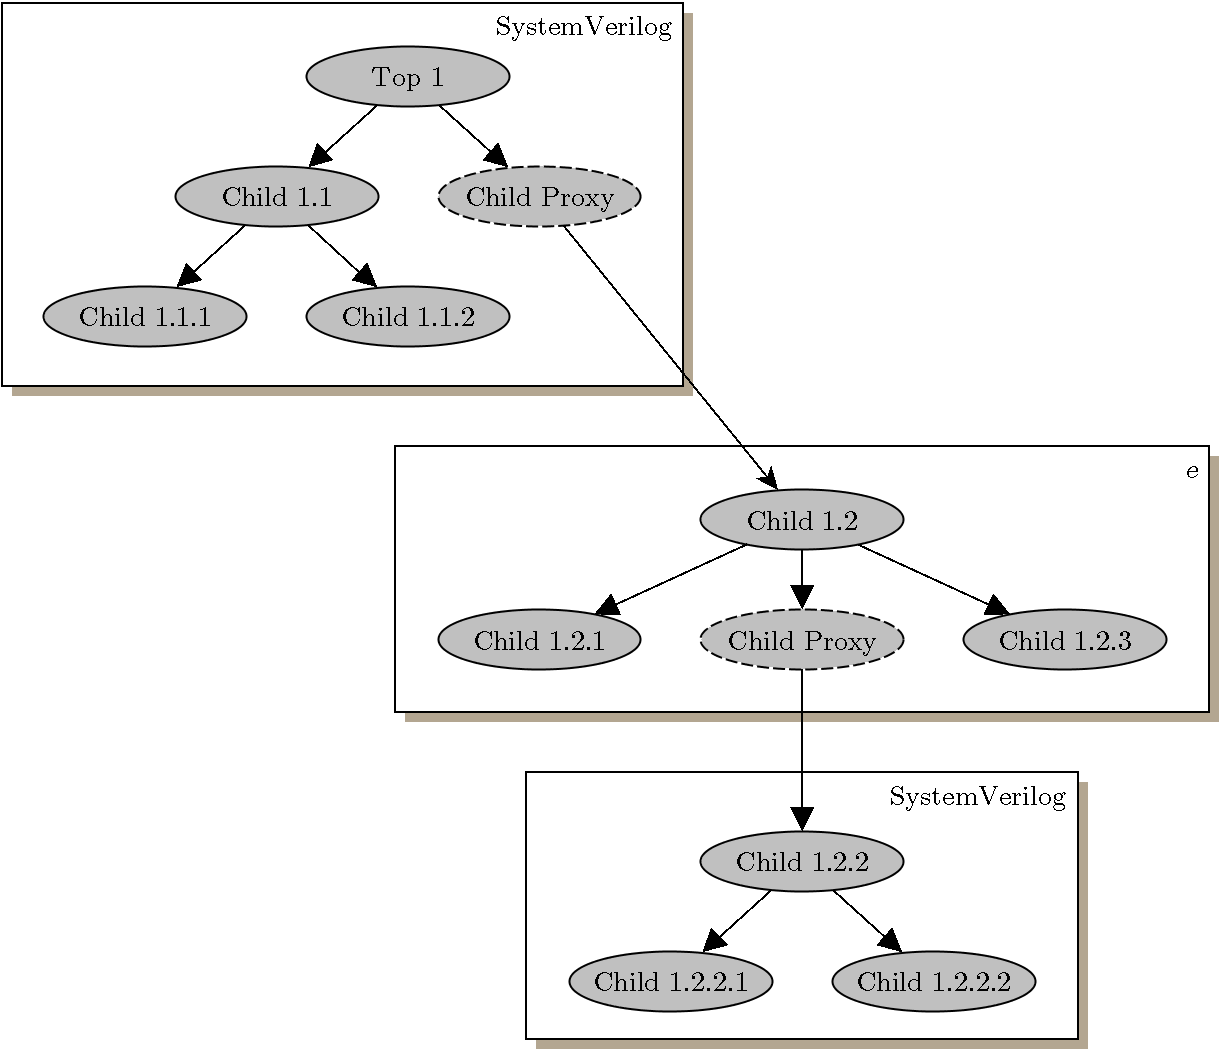
\includegraphics[width=1.0\textwidth,angle=0]{abb/UVM_ML_unified}
 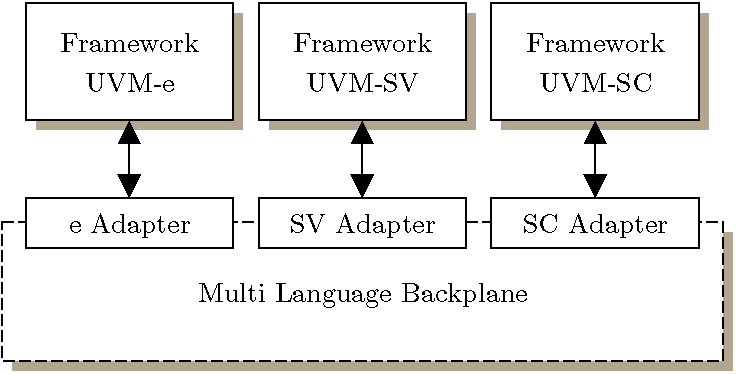
\includegraphics[scale=0.3]{abb/UVM_ML_architecture}
 \caption{UVM-ML architecture}
\label{fig:UVM_ML_architecture}
\end{figure}

The basic structure of the multi-language architecture is displayed in figure~\ref{fig:UVM_ML_architecture}. Each
framework accesses the backplane exclusively through its corresponding adapter. There are only the three adapters shown,
which are provided by the UVM-ML package, but it can be extended to support other frameworks as well.

\subsection{Integrate Multi-Language Functionality into Incisive Enterprise
Simulator}
At the current state of work multi-language support can be integrated into Cadence Incisive Enterprise Simulator via an open source package provided by Accellera Systems Initiative and developed jointly by AMD and Cadence Design
Systems. This package is called \emph{UVM-ML Open Architecture} and is provided as download on the Accellera website \cite{uvm_ml}.
For this report version 1.5.1 of the package was used. After downloading and extracting, it can be
installed via the provided install script called \lstinline$install_ies.csh$ and the following steps using \emph{C shell}:

\medskip
\lstset{language={}, numbers=none, escapechar=|}
\begin{lstlisting}
% setenv UVM_ML_HOME <install_dir>
% set path= (<path_to_irun> $path)
% source $UVM_ML_HOME/ml/install_ies.csh [--64bit] [--no-osci]
\end{lstlisting} 
\medskip 

Using \emph{Bourne shell} the corresponding commands are:

\medskip
\lstset{language={}, numbers=none, escapechar=|}
\begin{lstlisting}
% export UVM_ML_HOME=<install_dir>
% export PATH=<path_to_irun>:$PATH
% csh -c "source $UVM_ML_HOME/ml/install_ies.csh [--64bit] [--no-osci]"
\end{lstlisting} 
\medskip 

Due to some problems with the installation on \emph{Ubuntu} it is recommended to use an alternative distribution like
\emph{CentOS}. The environment variable \lstinline$UVM_ML_HOME$ needs to point to the root directory of the UVM-ML
package, which is \lstinline$UVM_ML-1.5.1$ for version 1.5.1. When already using IES, the standard setup script can be used
instead of manually setting the path environment variable to the \emph{irun} installation. While sourcing
\lstinline$install_ies.csh$ additional options can be used to control it. To install the environment on a 64 bit machine
instead of a 32 bit one use \lstinline$--64bit$. If only the adapters for UVM-SV, UVM-SystemC and
UVM-\textit{e} are required, UVM-ML can be build without the ASI-SystemC adapter via \lstinline$--no_osci$.\\
After this installation UVM-ML enables the creation of multi-language environments as well as running tests, which is
discussed in the following sections.

\subsection{Creating a Multi-Language Environment}
A verification environment typically consists of a system UVC containing
multiple subsystem UVCs, interface UVCs or module UVCs. These are composed in a
hierarchical way. With UVM-ML an environment can be constructed with components,
which are implemented in different frameworks. For example it could be composed
of an interface UVC implemented in UVM-SV and a module UVC in
UVM-\textit{e}. \\
When planing to create such a multi-language environment, there
are two possible approaches supported by UVM-ML to achieve this goal. Firstly an
\emph{unified hierarchy} can be created or alternatively a \emph{side-by-side}
environment. In an \emph{unified hierarchy} a child component implemented in one
verification language is instantiated from a parent component in another
verification language. In contrast, when creating a \emph{side-by-side} architecture,
the environment contains multiple tops.

\subsubsection{Creating an \emph{Unified Hierarchy} Environment}
To implement an \emph{unified hierarchy} each component which instantiates a
component of another framework needs to create and connect a proxy to
this component (this can be seen in figure~\ref{fig:UVM_ML_unified}). Then the
backplane applies operations which are performed on the proxy to the
corresponding component in the other verification language. This gives the
opportunity to use some of benefits of UVM-ML. It is possible to use a predefined
phasing in this environment, where phases like \lstinline$build$, \lstinline$connect$ or \lstinline$run$ are
performed depth-first to ensure that dependencies between the components of
different frameworks are resolved in the right way \cite{uvm_ml_ref}. Also sub-components can be
configured which increases the reusability of the environment, because when the
environment is included in some other environment, only the top component needs
to be configured and all sub-components are configured automatically. As a result of
this, it is recommended to implement such an environment.\\
Following it is described how to create a \emph{unified hierarchy} which
instantiates an UVM-SV component within an UVM-\textit{e} unit and vice versa.

\begin{figure}[htb]
 \centering
 %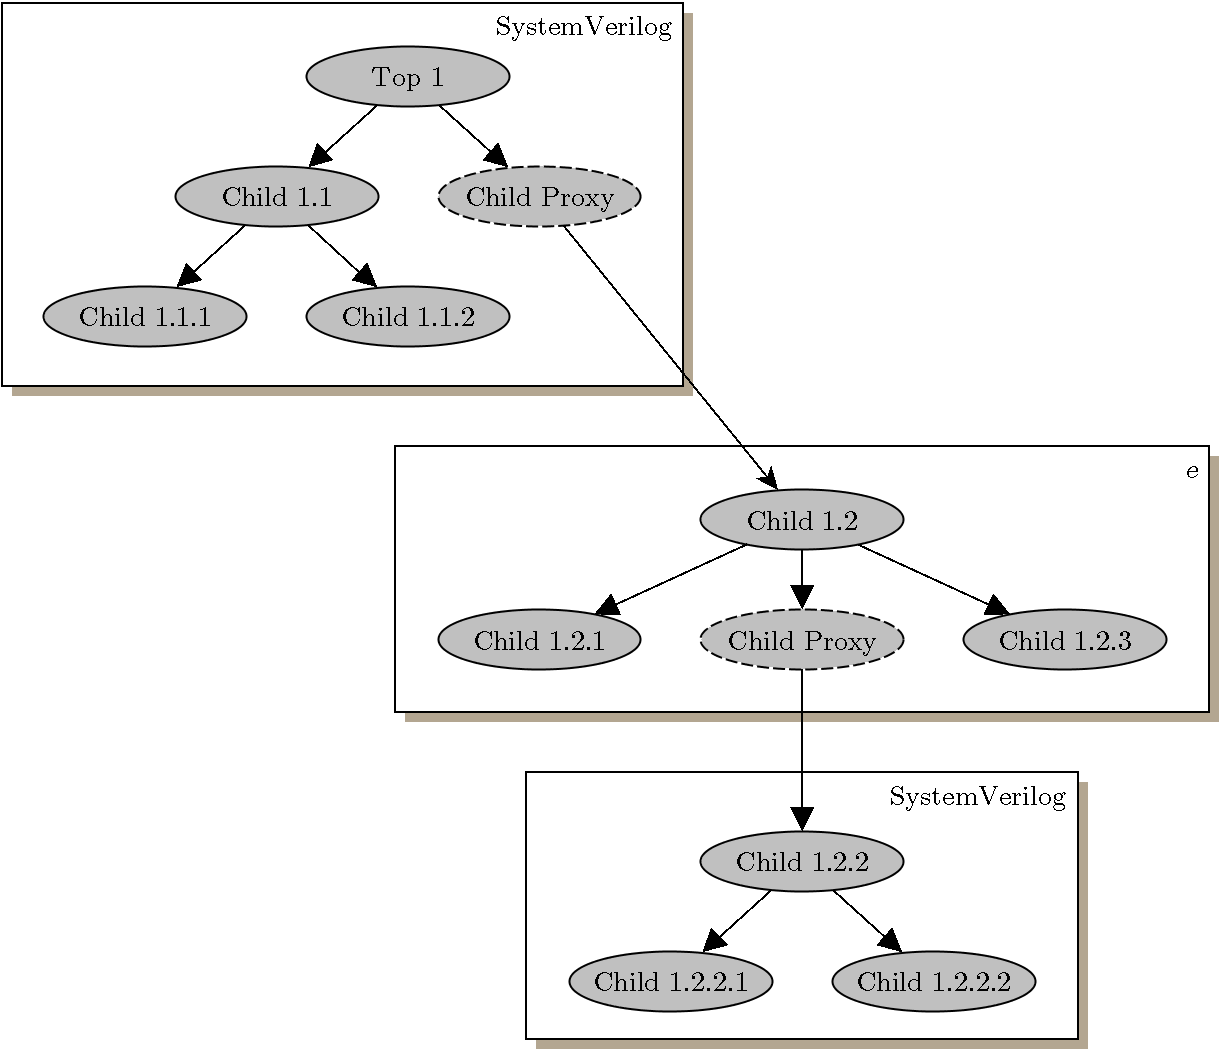
\includegraphics[width=1.0\textwidth,angle=0]{abb/UVM_ML_unified}
 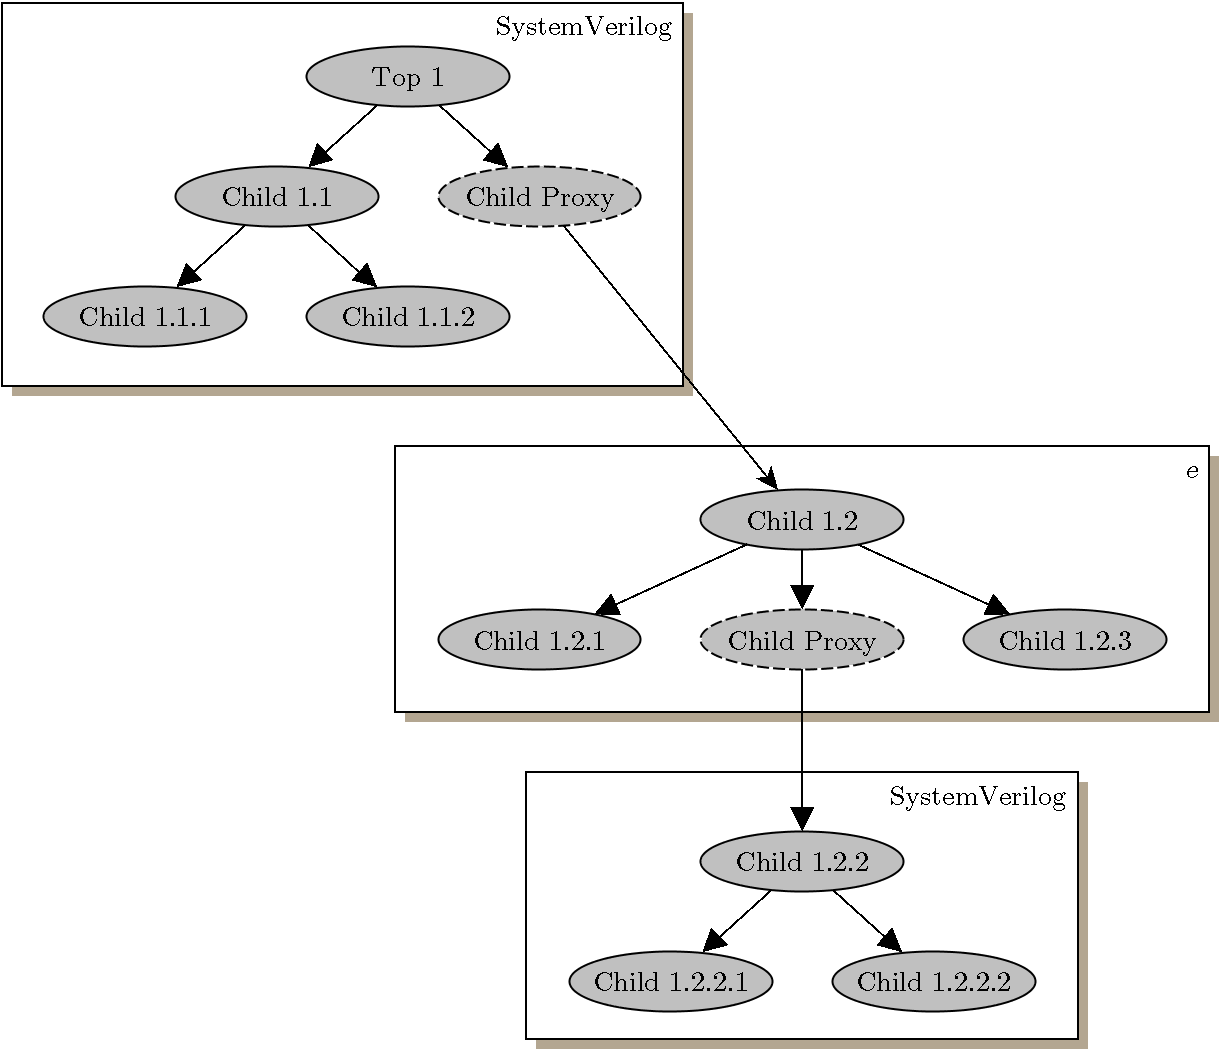
\includegraphics[scale=0.3]{abb/UVM_ML_unified}
 \caption{Structure of an \emph{unified hierarchy} environment}
\label{fig:UVM_ML_unified}
\end{figure}

\paragraph{Instantiating an UVM-SV Component within an UVM-\textit{e} Unit}
\label{sv_inside_e}
When instantiating an UVM-SV component within an UVM-\textit{e} unit,
it is necessary to instantiate a proxy unit inside the UVM-\textit{e} unit. After that the
proxy unit and the UVM-SV component need to be connected. \\
An example for the code of the extended UVM-SV component can be seen in
example~\ref{lst:SV_unified_sub}.
It is recommended to extend the UVM-SV component
(line~\ref{line_extend_component}) which will
be reused and then put all multi-language functionalities inside this new
component to ensure that the original component can still be used in
non-multi-language environments. The extended one needs to include the UVM
package (line~\ref{line_uvm_package}/\ref{line_uvm_macros}) as well as the adapter
package for UVM-SV (line~\ref{line_uvm_ml_package}).
After that all additional multi-language functionalities can be put inside the
class like configuring the sub-component (see section~\ref{ml_config}) or data
communication via TLM interfaces (see section~\ref{ml_tlm}).
\medskip
\lstset{language={SystemVerilog}, numbers=left, escapechar=|}
\begin{lstlisting}[frame=htrbl, caption={SystemVerilog: extended multi-language component}, label={lst:SV_unified_sub}]
import uvm_pkg::*;					|\label{line_uvm_package}|
`include "uvm_macros.svh"			|\label{line_uvm_macros}|
import uvm_ml::*;					|\label{line_uvm_ml_package}|

class ml_uvc_env extends uvc_env;			|\label{line_extend_component}|
  `uvm_component_utils(ml_uvc_env)
  function void build_phase(uvm_phase phase);
    // Additional multi-language functionalities
  endfunction : build_phase
endclass : ml_uvc_env
\end{lstlisting}
\medskip
Corresponding to the extensions in the UVM-SV component the UVM-\textit{e}
unit needs to include a proxy unit for the foreign component (see example~\ref{lst:e_unified_top}).
This can be done by instantiating an unit of type
\lstinline$child_component_proxy$ (line~\ref{line_uvm_ml_e_proxy}) which is a
predefined data type in the UVM-\textit{e} adapter.
Through constraining the proxy unit's \lstinline$type_name$ field
(line~\ref{line_uvm_ml_e_proxy_keep}) the
SystemVerilog component is integrated into the hierarchy. Thereby the string
needs to be composed of \lstinline$target_frmw_indicator:component_type_name$, where
\lstinline$target_frmw_indicator$ (case-insensitive) identifies the framework
of the instantiated foreign child component and can be \lstinline$SV$ for
UVM-SV, \lstinline$e$ for UVM-\textit{e} or \lstinline$SC$ for UVM-SystemC and
\lstinline$component_type_name$ is the type of the instantiated component.
\medskip
\lstset{language=e, numbers=left, escapechar=|}
\begin{lstlisting}[frame=htrbl, caption={\textit{e}: instantiating the UVM-SV component in the UVM-\textit{e} unit},
label={lst:e_unified_top}]
unit e_uvc_env {
  sv_uvc: child_component_proxy is instance;	|\label{line_uvm_ml_e_proxy}|
    keep sv_uvc.type_name == "SV:ml_uvc_env";|\label{line_uvm_ml_e_proxy_keep}| 
};
\end{lstlisting}

\paragraph{Instantiating an UVM-\textit{e} Unit Within an UVM-SV Component}
When reusing an UVM-\textit{e} unit inside of an UVM-SV component it is
necessary to integrate a proxy for the e unit within the UVM-SV
component and then connect both.\\
As shown in example~\ref{lst:SV_unified_top} this proxy component is created by
declaring a component of type \lstinline$uvm_component$ inside of the parent
component (line~\ref{line_sv_declare_proxy}). In the \lstinline$build_phase$ this proxy component is
instantiated via calling \lstinline$uvm_ml_create_component$ (line~\ref{line_sv_create_proxy}) with the following
syntax:
\medskip
\lstset{language={}, numbers=none, escapechar=|}
\begin{lstlisting}
function uvm_ml::child_component_proxy uvm_ml_create_component(
  string target_frmw_indicator,
  string component_type_name,
  string instance_name,
  uvm_component parent=null)
\end{lstlisting} 
\medskip
Where \lstinline$target_frmw_indicator$ indicates the framework adapter of the
foreign component (see section~\ref{sv_inside_e}),
\lstinline$component_type_name$ is the type of the foreign component according
to its declaration inside its framework, \lstinline$instance_name$ is the name
of the instance of the component proxy and \lstinline$parent$ is the handle of
the parent instance (\lstinline$this$ indicates the current component).\\
Because multi-language functionality is already integrated in UVM-\textit{e}, the child unit does not need any changes
to support the creation of an \emph{unified hierarchy} environment.
\medskip
\lstset{language=SystemVerilog, numbers = left, escapechar=|, breaklines=true}
\begin{lstlisting}[frame=htrbl, caption={SystemVerilog: instantiating an e unit}, label={lst:SV_unified_top}]
class testbench extends uvm_env;
  uvm_component e_uvc;|\label{line_sv_declare_proxy}|
  `uvm_component_utils(testbench)

  function void build_phase(uvm_phase phase);
    super.build_phase(phase);
    e_uvc = uvm_ml_create_component("e", "uvc_env_u", "e_uvc", this); |\label{line_sv_create_proxy}|
  endfunction
endclass : testbench
\end{lstlisting}

\subsubsection{Creating a \emph{Side-by-Side} Environment}

When there is no need to create an \emph{unified hierarchy} environment, UVM-ML supports also the ability to build an
environment with multiple tops as displayed in figure~\ref{fig:UVM_ML_side_by_side}. Here each tree inside of a
framework has its root instantiated as top component. This architecture is called \emph{side-by-side} and best
applicable when there is only limited synchronization required between the components of different frameworks. This is
indicated by the limitations of the architecture. It is not possible to use multi-language configuration as described in
section~\ref{ml_config}. Additionally the behavior of the phase execution is limited. Here each phase is first executed
completely on one tree before moving on to the next one. 

\begin{figure}[htb]
 \centering
 %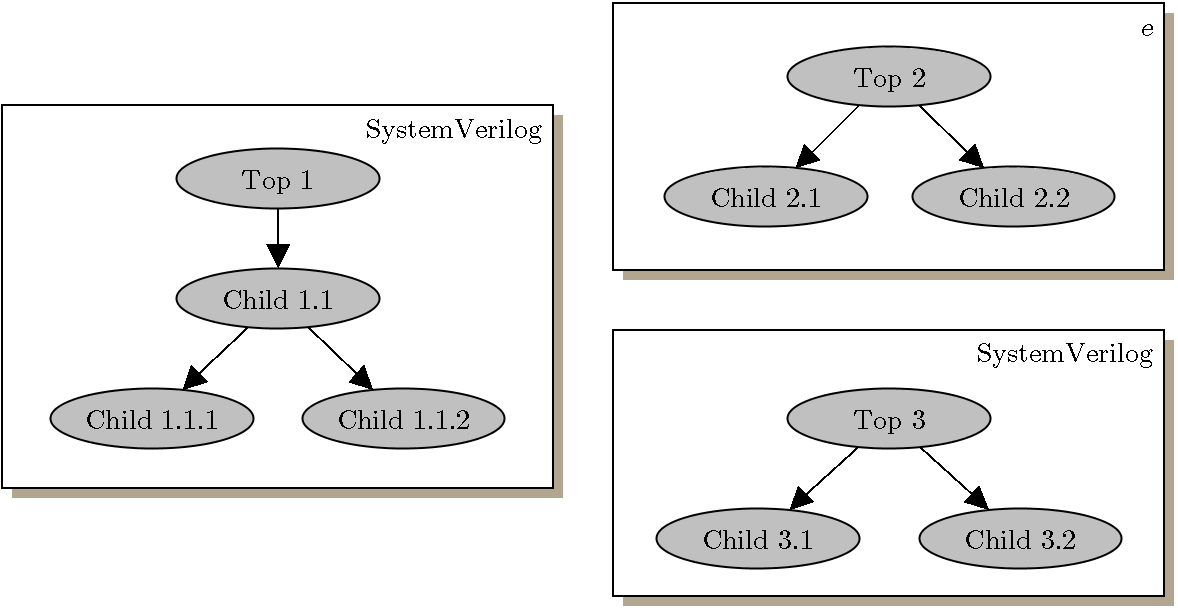
\includegraphics[width=1.0\textwidth,angle=0]{abb/UVM_ML_side_by_side}
 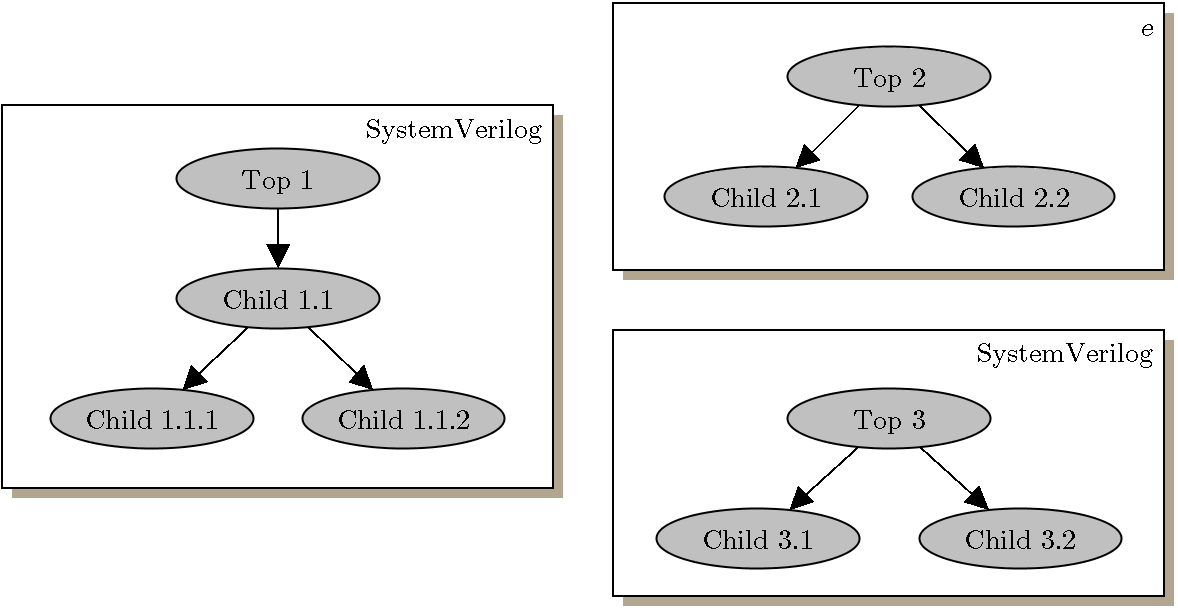
\includegraphics[scale=0.3]{abb/UVM_ML_side_by_side}
 \caption{Structure of a \emph{side-by-side} environment}
\label{fig:UVM_ML_side_by_side}
\end{figure}

\subsection{Mapping Data Items Across Frameworks }\label{type_mapping}
UVM-ML provides two options for data transfer between components of foreign frameworks. Firstly the configuration
database (section~\ref{ml_config}), which gives the ability to customize the structure of the multi-language
environment and secondly TLM communication (section~\ref{ml_tlm}) for ongoing transfer of transactions between foreign components.\\
Both of them require, that the types of the transferred transactions match in both frameworks as well as the
serialization and de-serialization needs to match to ensure data consistence for both communication partners.

\subsubsection{Type Mapping}
Type mapping in a multi-language environment means, that a user defined type, like a struct or class, in
one framework is mapped to a corresponding type definition in another foreign framework. So the multi-language
backplane needs to know, which type definitions shall be mapped onto each other. By default this is implicitly done by
looking for equal type names.\\
If type names differ, but the type descriptions should be mapped onto each other, the mapping can be done explicitly.
For this purpose both, the UVM-SV multi-language adapter as well as UVM-\textit{e} provide a function respectively
statement, which are shown below. Thereby \lstinline$frmw_indicator$ describes the framework, in which the type is
declared (\lstinline$sv$ for UVM-SV, \lstinline$e$ for UVM-\textit{e}) and \lstinline$type_name$ is the name
of the type within its framework.
\begin{itemize}
  \item{UVM-SV}
\lstset{language={}, numbers=none, escapechar=|}
\begin{lstlisting}
set_type_match("frmw_indicator:type_name", "frmw_indicator:type_name");
\end{lstlisting} 
  \item{UVM-\textit{e}}
\lstset{language={}, numbers=none, escapechar=|}
\begin{lstlisting}
uvm_ml_type_match "frmw_indicator:type_name" "frmw_indicator:type_name"
\end{lstlisting} 
\end{itemize}

An example for both multi-language adapters mapping functionality is shown in example~\ref{lst:SV_type_mapping}
respectively example~\ref{lst:e_type_mapping}, where the struct \lstinline$e_packet$ is mapped onto the class
\lstinline$sv_packet$. Take into account, that the explicit type mapping only needs to occur in one component, either in
the UVM-SV component (example~\ref{lst:SV_type_mapping}, line~\ref{line_sv_mapping}) or the
UVM-\textit{e} unit (example~\ref{lst:e_type_mapping}, line~\ref{line_e_mapping}).

\lstset{language=SystemVerilog, numbers = left, escapechar=|, breaklines=true}
\begin{lstlisting}[frame=htrbl, caption={SystemVerilog: mapping \lstinline$sv_packet$ onto \lstinline$e_packet$},
label={lst:SV_type_mapping}]
class sv_packet extends uvm_transaction;
  int data;
  
  `uvm_object_utils_begin(sv_packet)
    `uvm_field_int(data, UVM_ALL_ON)|\label{line_sv_physical}|
  `uvm_object_utils_end
endclass : sv_packet

class testbench extends uvm_env;
  function void build_phase(uvm_phase phase);
    super.build_phase(phase);
    void'(set_type_match("e:e_packet", "sv:sv_packet"));|\label{line_sv_mapping}|
  endfunction : build_phase
endclass : testbench
\end{lstlisting}

\lstset{language=e, numbers = left, escapechar=|, breaklines=true}
\begin{lstlisting}[frame=htrbl, caption={\textit{e}: mapping \lstinline$sv_packet$ onto \lstinline$e_packet$},
label={lst:e_type_mapping}]
struct e_packet like any_struct {
  %data : int;|\label{line_e_physical}|
};

uvm_ml_type_match "e:e_packet" "sv:sv_packet"|\label{line_e_mapping}|
\end{lstlisting}

\subsubsection{Serialization and De-Serialization}
When transactions are transmitted across multiple frameworks, their representation inside of one framework cannot
directly be transferred into a foreign framework. Even if they are composed of the same fields, the internal
representation differ between frameworks. Therefore transactions are firstly serialized into an universal bitstream,
then this bitstream is transmitted to the foreign framework and finally de-serialized to extract the transaction from
it.\\
UVM-SV as well as UVM-\textit{e} support default serialization and de-serialization. To use this
functionalities,  the order and type of fields in the transactions must match between the declarations. Only fields,
which are marked with a leading \lstinline$%$ are used for serialization and de-serialization in UVM-\textit{e} (see
example~\ref{lst:e_type_mapping}, line~\ref{line_e_physical} ) and other fields inside the struct are ignored. The same
occurs in UVM-SV for fields, if the \lstinline$`uvm_field_*$ macro is defined for them with the flag for
packing/unpacking set within the macro (see example~\ref{lst:SV_type_mapping}, line~\ref{line_sv_physical}).\\
If the default serialization and de-serialization cannot be applied to a transaction, manual ones can be created by
implementing \lstinline$do_pack()$ as well as \lstinline$do_unpack()$ for UVM-SV transactions and
\lstinline$pack()$ as well as \lstinline$unpack()$ for UVM-\textit{e}, but this is not further discussed in this report. 
\subsection{Configuring a Multi-Language Environment} \label{ml_config}
After building a multi-language environment it is often necessary to perform additional configurations before starting a
test. For example, setting an agent as passive respectively active or the number of resources available. In an
environment with an \emph{unified hierarchy} such configurations can be propagated from one framework tree
to all sub-trees in other frameworks. This is achieved by using the native UVM configuration constructs of each
framework, which are listed below:
\begin{itemize}
\item{UVM-SV:}
%\medskip
\lstset{language={}, numbers=none, escapechar=|}
\begin{lstlisting}
uvm_config_db#(T)::set()
uvm_config_db#(T)::get()
\end{lstlisting} 
%\medskip

\item{UVM-\textit{e}}
%\medskip
\lstset{language={}, numbers=none, escapechar=|}
\begin{lstlisting}
keep uvm_config_set()
keep uvm_config_get()
\end{lstlisting} 
%\medskip
\end{itemize}

Each framework maintains its own configuration database. These are synchronized automatically via the multi-language
backplane when a configuration is set. Thereby for getting the configuration information each framework just needs to
access its local database, which hides the multi-language functionality from each framework.

\subsubsection{\textit{e} Units Configuring UVM-SV Components}\label{e_config_sv}

When configuring UVM-SV components via UVM-\textit{e} units it is necessary to distinguish between two cases. Firstly
configuring it via primitive data types, where the data can directly be registered and obtained and secondly using
configuration objects, which requires to obtain the object using its base class followed by a cast to its proper data
type.\\
Since UVM-ML version~1.4.4 the generic UVM-SV syntax using \lstinline$uvm_config_db#(T)$ is supported, which
provides a more convenient option to configure user defined data types. 

\paragraph{Configuring UVM-SV Components using Primitive Data Types}\label{config_sv_primitive}

When data is passed from an UVM-\textit{e} unit to an UVM-SV component,
the UVM-\textit{e} unit needs to constrain \lstinline$uvm_config_set()$ as shown in example~\ref{lst:e_set_int}
line~\ref{line_e_set_int}. In this example the value \lstinline$16'h7fff$ is assigned to the variable
\lstinline$field_1$ in all components, which contain the letters \lstinline$uvc_env$ in their full path.

\lstset{language=e, numbers = left, escapechar=|, breaklines=true}
\begin{lstlisting}[frame=htrbl, caption={\textit{e}: register an integer in configuration database},
label={lst:e_set_int}]
extend testbench {
    keep uvm_config_set("*uvc_env*", "field_1", 16'h7fff);|\label{line_e_set_int}|
};
\end{lstlisting}

After the configuration is set in the database by the UVM-\textit{e} unit, the UVM-SV component needs to get
the value from its database. When it is a primitive data type like an integer as in example~\ref{lst:SV_get_int},
the corresponding \lstinline$uvm_config_*::get()$ method should be used as shown in line~\ref{line_sv_get_int}. Here the
value of \lstinline$field_1$ registered for this component in the database is assigned to the variable with the same
name, \lstinline$field_1$.\\
When the field was specified with the corresponding \lstinline$uvm_field_*$ macro, calling
\lstinline$uvm_config_*::get()$ is not required. Its value is automatically retrieved from the configuration database.

\lstset{language=SystemVerilog, numbers = left, escapechar=|, breaklines=true}
\begin{lstlisting}[frame=htrbl, caption={SystemVerilog: getting an integer from configuration database},
label={lst:SV_get_int}]
class ml_uvc_env extends uvc_env;
  int field_1;|\label{line_sv_declare_int}|
  function void end_of_elaboration_phase(uvm_phase phase);
  	super.end_of_elaboration_phase(phase);
    void'(uvm_config_int::get(this, "", "field_1", field_1));|\label{line_sv_get_int}|
  endfunction : end_of_elaboration_phase
endclass
\end{lstlisting}

\paragraph{Configuring UVM-SV Components using Objects}\label{e_config_sv_object}

When using configuration objects instead of primitive data types, the UVM-\textit{e} unit can access its configuration
database the same way as with a primitive data type as shown in example~\ref{lst:e_set_object}. In this example
an object of type \lstinline$data$ is created (line~\ref{line_e_declare_object}) and then registered in the
configuration database (line~\ref{line_e_set_object}) the same way as for primitive data types
(section~\ref{config_sv_primitive}).

\lstset{language=e, numbers = left, escapechar=|, breaklines=true}
\begin{lstlisting}[frame=htrbl, caption={e: register an object in configuration database}, label={lst:e_set_object}]
struct data {
  % addr    : int;
  % trailer : int;
  % txt     : string;
};

unit u {
  my_sv_child: child_component_proxy is instance;
    keep my_sv_child.type_name == "SV:test";
  
  d : data;|\label{line_e_declare_object}|
    keep d.addr    == 10;
    keep d.trailer == 20;
    keep d.txt     == "config object msg";

  keep uvm_config_set("my_sv_child","conf_data",d);|\label{line_e_set_object}|
};
\end{lstlisting}
The difference between configuring an UVM-SV component using a primitive data type compared to an object
is displayed in example~\ref{lst:SV_get_object}. Additionally to the declaration of the object in
line~\ref{line_sv_declare_object} another one of type \lstinline$uvm_object$ is required
(line~\ref{line_sv_declare_data}). Configuration objects need to be derived from this base type as shown in
line~\ref{line_sv_class_object} (\lstinline$uvm_transaction$ inherits from \lstinline$uvm_object$).\\
When the field of type \lstinline$uvm_object$ was specified with the \lstinline$uvm_field_object$ macro, calling
\lstinline$uvm_config_object::get()$ is not required. Its value is automatically retrieved from the configuration
database and can then be cast directly to the proper data type.\\
As mentioned previously, the generic syntax using \lstinline$uvm_config_db#(T)$ can be used to obtain configuration
objects as an alternative to \lstinline$uvm_config_object$.
The benefit of this approach is, that an additional cast after getting the object is not required as shown in
line~\ref{line_sv_get_user_object}. The object with the user defined type \lstinline$data$ is directly obtained from
the database, so line \ref{line_sv_declare_object}, \ref{line_sv_get_object} and \ref{line_sv_cast_object} are replaced
by this single line of code.

\lstset{language=SystemVerilog, numbers = left, escapechar=|, breaklines=true}
\begin{lstlisting}[frame=htrbl, caption={SystemVerilog: getting a configuration object}, label={lst:SV_get_object}]
class data extends uvm_transaction;|\label{line_sv_class_object}|
  int addr;
  int trailer;
  string txt;
  
  `uvm_object_utils_begin(data)
    `uvm_field_int(   addr,    UVM_ALL_ON)
    `uvm_field_int(   trailer, UVM_ALL_ON)
    `uvm_field_string(txt,     UVM_ALL_ON)
  `uvm_object_utils_end
endclass

class test extends uvm_env;
  uvm_object tmp_obj;|\label{line_sv_declare_object}|
  data conf_data;|\label{line_sv_declare_data}|
  
  function void build_phase(uvm_phase phase);
    super.build_phase(phase);
    void'(uvm_config_object::get(this,"","conf_data", tmp_obj));|\label{line_sv_get_object}|
    assert($cast(conf_data,tmp_obj)!=0);|\label{line_sv_cast_object}|
    //-- alternativly uvm_config_db can be used
    //void'(uvm_config_db#(data)::get(this,"","conf_data",conf_data));|\label{line_sv_get_user_object}|
  endfunction
endclass
\end{lstlisting}
It is important that the declarations of the configuration object in both verification languages are mapped to each
other. This includes the number and order of variables as well as the name of the type definition. For more information
on type mapping see section~\ref{type_mapping}.

\subsubsection{SystemVerilog Components Configuring UVM-\textit{e} Units}
Similar to section~\ref{e_config_sv} UVM-SV components can configure UVM-\textit{e} units via the
configuration database. The syntax remains the same, just the part of getting respectively setting is switched for both
frameworks. The field that should be configured has to be registered in the database by the UVM-SV
component prior to creating the sub-component. Then the UVM-\textit{e} unit needs to be constrained using
\lstinline$uvm_config_get()$ to receive the value from the configuration database.

\paragraph{Configuring UVM-\textit{e} Units using Primitive Data Types}
When configuring an UVM-\textit{e} unit via an UVM-SV component, the component needs to register the value in
the configuration database by calling \lstinline$uvm_config_*::set()$. This needs to be
done before creating the foreign sub-component using the field. That is necessary so the constraint solver of
\textit{e} can access the database, when the unit is instantiated. This is displayed in example~\ref{lst:SV_set_int},
that shows the UVM-SV component, configuring a field of type integer within an UVM-\textit{e} unit. Firstly
the integer is registered at the configuration database in line~\ref{line_sv_set_int}. After that the component, which uses this registered field, is created in
line~\ref{line_sv_comp_int}.

\lstset{language=SystemVerilog, numbers = left, escapechar=|, breaklines=true}
\begin{lstlisting}[frame=htrbl, caption={SystemVerilog: register an integer in configuration database},
label={lst:SV_set_int}]
class uvc_env extends uvm_env;
  uvm_component e_uvc;
  
  function void build_phase(uvm_phase phase);
    super.build_phase(phase);
    uvm_config_int::set(this,"*e_uvc*","field_1", 10);|\label{line_sv_set_int}|
    e_uvc = uvm_ml_create_component("e", "uvc_env_u", "e_uvc", this);|\label{line_sv_comp_int}|
  endfunction : build_phase
endclass : uvc_env
\end{lstlisting}

Once the field is registered in the configuration database, the UVM-\textit{e} unit just needs to constrain
\lstinline$uvm_config_get$, as shown in example~\ref{lst:e_get_int}, line~\ref{line_e_get_int}. After that the value can
be used inside of the unit.

\lstset{language=e, numbers = left, escapechar=|, breaklines=true}
\begin{lstlisting}[frame=htrbl, caption={e: getting an integer from configuration database}, label={lst:e_get_int}]
unit uvc_env_u {
  field_1 : int;
  keep soft uvm_config_get(field_1); |\label{line_e_get_int}|
};
\end{lstlisting}
\paragraph{Configuring UVM-\textit{e} Units using Objects}
Like UVM-SV components, UVM-\textit{e} units can be configured via objects. An example for registering an
object in the configuration database via an UVM-SV component is described in
example~\ref{lst:SV_set_object}. Firstly the component needs to declare the type of the object
(line~\ref{line_sv_class_object_2}). After registering the object at the configuration database with
\lstinline$uvm_config_db#(T)::set()$ (line~\ref{line_sv_set_user_object}), the foreign child component, which uses the
configuration object, can be created (line~\ref{line_sv_comp_object_2}).

\lstset{language=SystemVerilog, numbers = left, escapechar=|, breaklines=true}
\begin{lstlisting}[frame=htrbl, caption={SystemVerilog: register an object in configuration database},
label={lst:SV_set_object}]
class data extends uvm_transaction;|\label{line_sv_class_object_2}|
  int addr;
  int trailer;
  string txt;
  
  `uvm_object_utils_begin(data)
    `uvm_field_int(   addr,    UVM_ALL_ON)
    `uvm_field_int(   trailer, UVM_ALL_ON)
    `uvm_field_string(txt,     UVM_ALL_ON)
  `uvm_object_utils_end
endclass

class test extends uvm_env;
  uvm_component my_e_child; 
  data conf_data;|\label{line_sv_declare_data_2}|
  
  function void build_phase(uvm_phase phase);
    super.build_phase(phase);
    conf_data.addr = 10;
    conf_data.trailer = 20;
    conf_data.txt = "config object msg"
    void'(uvm_config_db#(data)::set(this, "my_e_child", "conf_data", conf_data));|\label{line_sv_set_user_object}|
    my_e_child = uvm_ml_create_component("e", "child_u", "my_e_child", this);|\label{line_sv_comp_object_2}|
  endfunction
endclass
\end{lstlisting}

Similar to the UVM-SV component, the type of the configuration object needs to be declared in the
\textit{e} unit, too (line~\ref{line_e_declare_object_2}). These declarations need to be mapped onto each other. This
means that they need the same number and order of fields as well as matching type names. See section~\ref{type_mapping}
for more information about type mapping.\\
If the declarations match, the UVM-\textit{e} unit simply needs to instantiate the configuration object
(line~\ref{line_e_inst_object_2}) and constrain \lstinline$uvm_config_get()$ to obtain the object from the
configuration database.

\lstset{language=e, numbers = left, escapechar=|, breaklines=true}
\begin{lstlisting}[frame=htrbl, caption={e: getting an object from configuration database}, label={lst:e_get_object}]
struct data {|\label{line_e_declare_object_2}|
  % addr    : int;
  % trailer : int;
  % txt     : string;
};

unit child_u {
  conf_data : data;|\label{line_e_inst_object_2}|
    keep soft uvm_config_get(conf_data);
};
\end{lstlisting}
\subsubsection{Connecting the Interface UVCs to the DUT}
Another configuration task when creating a multi-language environment is connecting the interface UVC to the DUT. The configuration database can also be used for this, if the interface UVC is implemented in a foreign framework. Following is discribed, how to configure the interface of an UVM-SV respectively the signal map of an UVM-\textit{e} interface UVC in a multi-language environment.
\paragraph{Configuring the UVM-SV Interface}
When a UVM-SV interface UVC is instantiated inside of an UVM-e component, the virtual interface of the interface UVC cannot be connected to the DUT inside of an \lstinline$inital$ block, because these blocks are executed after UVM-ML has executed the elaboration phases. Therefore a function is defined registering the interface in the configuration database (example~\ref{lst:SV_config_interface}, line~\ref{line_sv_function_vif}). Thereby the interface UVC is instantiated directly under \lstinline$sys$ and can obtain the interface from the database by calling \lstinline$uvm_config_db#(T)::get()$. The previously defined function is then executed in a static initialization call (line~\ref{line_sv_call_function_vif}).
\lstset{language=SystemVerilog, numbers = left, escapechar=|, breaklines=true}
\begin{lstlisting}[frame=htrbl, caption={SystemVerilog: configuring the UVM-SV interface},
label={lst:SV_config_interface}]
module tb;
  uvc_if inf(...);
	
  function bit set_vif(virtual uvc_if vif);|\label{line_sv_function_vif}|
    uvm_config_db#(virtual uvc_if)::set(null,"sys.sv_uvc*","vif",vif);|\label{line_sv_set_db_vif}|
    return 1;
  endfunction

  bit res = set_vif(inf);|\label{line_sv_call_function_vif}|
endmodule : tb
\end{lstlisting}
\paragraph{Configuring the UVM-\textit{e} Signal Map}
When creating a multi-language environment with a UVM-\textit{e} interface UVC, the simple ports of the signal map are connected to the DUT using the configuration database. In example~\ref{lst:SV_set_smp} the \lstinline$hdl_path()$ for the signal map and simple ports inside of it as well as the \lstinline$agent()$ are registered in the configuration database by the top level UVM-SV component. The base \lstinline$hdl_path()$ for the signal map is registered in line~\ref{line_sv_smp_path}. It consists of the string representing the name of the top level module of the DUT. Following the \lstinline$agent()$ is set in line~\ref{line_sv_smp_agent}. Thereby \lstinline$"SV"$ indicates, that the top level module of the DUT is implemented in SystemVerilog. After that the \lstinline$hdl_path()$ for each simple port is registered, exemplarily shown for a single port in line~\ref{line_sv_port_path}, with the registered string beeing the full path of the DUT signal without the top level module, which is set for the signal map (line~\ref{line_sv_smp_path}).
Finally the foreign interface UVC containing the signal map is instantiated in line~\ref{line_sv_create_smp}, after all necessary entries are registered in the configuration database.
\lstset{language=SystemVerilog, numbers = left, escapechar=|, breaklines=true}
\begin{lstlisting}[frame=htrbl, caption={SystemVerilog: configuring the simple ports of the UVM-\textit{e} signal map},
label={lst:SV_set_smp}]
class tb extends uvm_env;
  uvm_component e_uvc;
  //use uvm_component_utils macro here and implement the constructor

  function void build_phase(uvm_phase phase);
    super.build_phase(phase);
    uvm_config_string::set(this, "e_uvc.smp", "hdl_path()",          "~/tb_top");|\label{line_sv_smp_path}|
    uvm_config_string::set(this, "e_uvc.smp", "agent()",             "SV");|\label{line_sv_smp_agent}|
    uvm_config_string::set(this, "e_uvc.smp", "signal_1_p_hdl_path", "signal_1");|\label{line_sv_port_path}|
    //...
    e_uvc = uvm_ml_create_component("e", "uvc_env_u", "e_uvc", this);|\label{line_sv_create_smp}|
  endfunction : build_phase
endclass : tb
\end{lstlisting}
The next step in connecting the signal map of the interface UVC is to obtain the previously registered entries from the configuration database. The definition of the signal map of the interface UVC is displayed in example~\ref{lst:e_get_smp} line~\ref{line_e_smp}. Again it contains only a single examplary simple port. After that, the extended signal map is shown using the configuration database to connect the simple port to the DUT. Firstly a string is created for each simple port to store the path obtained from the database (line~\ref{line_e_declare_path_string}). After that the database is accessed to get the \lstinline$hdl_path()$ and \lstinline$agent()$ of the top level module of the DUT (line~\ref{line_e_get_smp_path}/\ref{line_e_get_smp_agent}). Eventually the \lstinline$hdl_path()$ of the simple port is obtained (line~\ref{line_e_get_port_string}) and constrained (line~\ref{line_e_set_port}). The full path is then automatically composed of the \lstinline$hdl_path()$ of the signal map and simple port.
\lstset{language=e, numbers = left, escapechar=|, breaklines=true}
\begin{lstlisting}[frame=htrbl, caption={\textit{e}: getting the simple port configuration of the UVM-\textit{e} signal map},
label={lst:e_get_smp}]
unit signal_map_u like uvm_signal_map {|\label{line_e_smp}|
  signal_1_p: inout simple_port of uint(bits: 4) is instance;
  //...
  keep HDL_SIGNAL_PATH is all of {
    soft signal_1_p.hdl_path() == "signal_1";
    //...
  };
};

extend signal_map_u {|\label{line_e_extend_smp}|
  signal_1_p_hdl_path : string;|\label{line_e_declare_path_string}|
  //...

  keep uvm_config_get(hdl_path());|\label{line_e_get_smp_path}|
  keep uvm_config_get(agent());|\label{line_e_get_smp_agent}|

  keep ML_HDL_SIGNAL_PATH is all of {
    uvm_config_get(signal_1_p_hdl_path);|\label{line_e_get_port_string}|
    signal_1_p.hdl_path() == value(signal_1_p_hdl_path);|\label{line_e_set_port}|
    //...
  };
}; 
\end{lstlisting}
\subsection{Data Communication in a Multi-Language Environment} \label{ml_tlm}
Additionally to the configuration database, UVM-ML uses TLM communication to manage the communication between components
of different frameworks. While communication via the configuration database only occurs once per item to build the
structure of the testbench, TLM communication is used to establish ongoing communication between components during the
test. Data transfer by use of UVM-ML TLM communication is achieved by serializing transactions sending the resulting
bitstream to the destination component via the connected port and after that de-serializing it there.\\
For this it is required, that the backplane knows, which types are mapped onto each other. Also the serialization and
de-serialization need to match, so the same transaction is available at both components. This implies, that the number
and order of fields in the user defined types have to be consistent.
Here it is discussed how to establish TLM communication on the example of TLM analysis ports. For more information on
type mapping see section~\ref{type_mapping}.\\
When it is ensured, that both frameworks handle compatible data items, TLM analysis ports have to be implemented in each
component including the \lstinline$write()$ method of the receiving TLM port. After the ports are instantiated they
are registered at their framework adapter. For UVM-SV this is done by calling
\lstinline$uvm_ml::tlm1::register()$ and for UVM-\textit{e} the port is bind to external by constraining \lstinline$bind()$.
Finally the ports are connected via \lstinline$uvm_ml::connect()$ for UVM-SV or
\lstinline$uvm_ml.connect_names()$ for UVM-\textit{e}. This should only be done once, either at the
SystemVerilog component or the UVM-\textit{e} unit.
\begin{itemize}
\item{UVM-SV:}
%\medskip
\lstset{language={}, numbers=none, escapechar=|}
\begin{lstlisting}
static function void uvm_ml::ml_tlm1#(T)::register(port);

function bit uvm_ml::connect(
  string producer_path,
  string consumer_path);
\end{lstlisting} 
%\medskip

\item{UVM-\textit{e}}
%\medskip
\lstset{language={}, numbers=none, escapechar=|}
\begin{lstlisting}
keep bind(port, external);

uvm_ml.connect_names(
  producer_path : string,
  consumer_path : string) : bool;
\end{lstlisting} 
%\medskip
\end{itemize}

Following examples for sending transactions from UVM-\textit{e} units to UVM-SV components and
vice versa are provided to show, how to utilize the above introduced TLM functionalities for multi-language
environments.
\subsubsection{\textit{e} Units Sending Transactions to UVM-SV Components}
In example~\ref{lst:SV_TLM_consumer} is the implementation of a TLM implementation port in UVM-SV
displayed. After declaring (line~\ref{line_sv_imp_declare}) and instantiating (line~\ref{line_sv_imp_inst}) the port, it
is registered at the UVM-SV multi-language adapter (line~\ref{line_sv_imp_reg}).
\lstset{language=SystemVerilog, numbers = left, escapechar=|, breaklines=true}
\begin{lstlisting}[frame=htrbl, caption={SystemVerilog: consumer side of a TLM connection},
label={lst:SV_TLM_consumer}]
class mod_monitor extends uvm_monitor;
  uvm_analysis_imp#(packet, mod_monitor) in_port;|\label{line_sv_imp_declare}|
  
  `uvm_component_utils(mod_monitor)
  
  function new(string name="mod_monitor", uvm_component parent);
    super.new(name, parent);
    in_port = new("in_port", this);|\label{line_sv_imp_inst}|
  endfunction 
  
  function void phase_ended(uvm_phase phase);
    if(phase.get_name() == "build") begin
      uvm_ml::ml_tlm1#(packet)::register(in_port);|\label{line_sv_imp_reg}|
    end
  endfunction : phase_ended
  
  virtual function void write(packet pkt);|\label{line_sv_imp_write}|
  //...
  endfunction : write
endclass
\end{lstlisting}
The corresponding UVM-\textit{e} producer is shown in example~\ref{lst:e_TLM_producer}. Its TLM port is implemented in
line~\ref{line_e_port_inst} and following registered by constraining \lstinline$bind()$ in line~\ref{line_e_port_reg}.
After both components are instantiated under \lstinline$sys$, their TLM ports are connected in line~\ref{line_e_connect}.
\lstset{language=e, numbers = left, escapechar=|, breaklines=true}
\begin{lstlisting}[frame=htrbl, caption={\textit{e}: producer side of a TLM connection},
label={lst:e_TLM_producer}]
unit inf_monitor like uvm_monitor {
  out_port : out interface_port of tlm_analysis of packet is instance;|\label{line_e_port_inst}|
    keep soft bind(out_port, external);|\label{line_e_port_reg}|
};

extend sys {
  e_inf_monitor  : inf_monitor is instance;
  sv_mod_monitor : child_component_proxy is instance;
    keep sv_mod_monitor.type_name == "sv:mod_monitor";
  
    
  connect_ports() is also {
    uvm_connect_names("sys.e_inf_monitor.outport", append(sv_mod_monitor.e_path(), ".in_port"));|\label{line_e_connect}|
  };  
};
\end{lstlisting}

\subsubsection{SystemVerilog Components Sending Transactions to UVM-\textit{e} Units}
Now the functionalities of consumer and producer are switched between both frameworks, so the TLM implementation port is
realized in UVM-\textit{e} (example~\ref{lst:e_TLM_consumer}). It is instantiated in line~\ref{line_e_imp_inst} followed
by its registration in line~\ref{line_e_imp_reg}.
\lstset{language=e, numbers = left, escapechar=|, breaklines=true}
\begin{lstlisting}[frame=htrbl, caption={\textit{e}: consumer side of a TLM connection},
label={lst:e_TLM_consumer}]
unit mod_monitor like uvm_monitor {
  in_port : in interface_port of tlm_analysis of packet is instance;|\label{line_e_imp_inst}|
    keep soft bind(out_port, external);|\label{line_e_imp_reg}|
    
  write(pkt : packet) is {|\label{line_e_imp_write}|
  //...
  };
};
\end{lstlisting}
The producer is shown in example~\ref{lst:SV_TLM_producer}. Its TLM port is declared in line~\ref{line_sv_port_declare}
and instantiated in line~\ref{line_sv_port_inst}. After that it is registered at the framework adapter in
line~\ref{line_sv_port_reg}. Finally both monitors are instantiated (line~\ref{line_sv_inst_monitors}) and their ports are connected (line~\ref{line_sv_con}).
\lstset{language=SystemVerilog, numbers = left, escapechar=|, breaklines=true}
\begin{lstlisting}[frame=htrbl, caption={SystemVerilog: producer side of a TLM connection},
label={lst:SV_TLM_producer}]
class inf_monitor extends uvm_monitor;
  uvm_analysis_port#(packet) out_port;|\label{line_sv_port_declare}|
  
  `uvm_component_utils(inf_monitor)
  
  function new(string name="inf_monitor", uvm_component parent);
    super.new(name, parent);
    out_port = new("out_port", this);|\label{line_sv_port_inst}|
  endfunction 
  
  function void phase_ended(uvm_phase phase);
    if(phase.get_name() == "build") begin
      uvm_ml::ml_tlm1#(packet)::register(out_port);|\label{line_sv_port_reg}|
    end
  endfunction : phase_ended
endclass

class env extends uvm_env;
  inf_monitor   sv_inf_monitor;
  uvm_component e_mod_monitor;
  
  `uvm_component_utils(env)
  
  function void build_phase(uvm_phase phase);|\label{line_sv_inst_monitors}|
    super.build_phase(phase);
    sv_inf_monitor = inf_monitor::type_id::create("sv_inf_monitor", this);
    e_mod_monitor  = uvm_ml_create_component("e", "mod_monitor", "e_mod_monitor", this); 
  endfunction : build_phase
  
  function void connect_phase(uvm_phase phase);
    uvm_ml::connect(sv_inf_monitor.get_full_name(), {get_full_name(),".e_mod_monitor.in_port"});|\label{line_sv_con}|
    endfunction : connect_phase
\end{lstlisting}

\subsection{Sequence Layering in a Multi-Language Environment}
The last step in creating a fully functional multi-language testbench is the stimuli generation. There are two typical
use cases for handling a sequence library implemented in a foreign framework. Firstly configuring the default sequence
of the sequencer contained in the foreign sub-component via the top level component, which requires minimal interaction between
these components. The second case requires ongoing communication between the sequences implemented in different
frameworks. Here a virtual sequence implemented at the top level continuously executes sequences of the sub-component.
Following is discussed, which extensions are required to support the use of foreign sequences.

\subsubsection{Configuring the Default Sequence}
The simplest way to use foreign sequences is to configure the default sequence of the sequencer included in the foreign
sub-component by using the configuration databases of both frameworks (see section~\ref{ml_config} for more detailed
information about the configuration databases). This determines, which sequence is started when the test begins.

\paragraph{UVM-\textit{e} Configuring the UVM-SV Default Sequence}
Example~\ref{lst:SV_get_default_sequence} shows, which changes are necessary in the UVM-SV sub-component to make its default sequence configurable via a foreign UVM-\textit{e} unit. The communication between the foreign components is done by registering the name of the sequence at the configuration database. Therefore a variable for this string has to be defined (line~\ref{line_sv_seq_name_var}). Following it is used to get the name of the sequence from the database in line~\ref{line_sv_get_seq_name}. Afterwards the sequence is obtained from the factory by searching for it with the provided name (line~\ref{line_sv_find_seq_by_name}). Finally this sequence is used to set the default sequence of the sequencer included in the agent, which is contained in the base class of this multi-language component (line~\ref{line_sv_set_default_seq}).   

\lstset{language=SystemVerilog, numbers = left, escapechar=|, breaklines=true}
\begin{lstlisting}[frame=htrbl, caption={SystemVerilog: getting the default sequence from configuration database},
label={lst:SV_get_default_sequence}]
class ml_uvc_env extends uvc_env;
  string seq_name; |\label{line_sv_seq_name_var}|
  
  function void build_phase(uvm_phase phase);
    uvm_factory factory = uvm_factory::get();|\label{line_sv_get_factory_handle}|
    uvm_object_wrapper seq_wrap;
    super.build_phase(phase);
    void'(uvm_config_string::get(this, "", "seq_name", seq_name));|\label{line_sv_get_seq_name}|
    seq_wrap = factory.find_by_name(seq_name);|\label{line_sv_find_seq_by_name}|
    uvm_config_db#(uvm_object_wrapper)::set(this, "agent.sequencer.run_phase", "default_sequence", seq_wrap);|\label{line_sv_set_default_seq}|
    endfunction
endclass : ml_uvc_env
\end{lstlisting}
The UVM-\textit{e} unit needs to provide the name of the sequence used to configure the default sequence of the foreign sequencer. For this purpose the name is registered at the configuration database in line~\ref{line_e_set_default_seq} of example~\ref{lst:e_set_default_sequence}.
\lstset{language=e, numbers = left, escapechar=|, breaklines=true}
\begin{lstlisting}[frame=htrbl, caption={\textit{e}: setting the default sequence via configuration database},
label={lst:e_set_default_sequence}]
extend sys {
  sv_uvc : child_component_proxy is instance;
    keep sv_uvc.type_name == "SV:ml_uvc_env"
    keep uvm_config_set("sv_uvc", "seq_name", "seq")|\label{line_e_set_default_seq}|
};
\end{lstlisting}
\paragraph{UVM-SV Configuring the UVM-\textit{e} Main Sequence}
Reversed the configuration database can be used to configure the \lstinline$main$ sequence of an UVM-\textit{e} unit through the enclosing UVM-SV component. Therefore the sequence driver of the sub-component has to be extended by a string variable, which is shown in line~\ref{line_e_get_seq_name} of example~\ref{lst:e_get_main_sequence}. It is used to store the name of the sequence, which is received from the configuration database in line~\ref{line_e_get_seq_name}. Afterwards the \lstinline$main$ sequence is extended, so its \lstinline$kind$-field can be constrained to equal the sequence identified by the previously received string. It is necessary to mention, that \lstinline$driver$ refers to the \emph{sequence driver} of UVM-\textit{e} and should not be mistaken with the \emph{driver} class of UVM-SV. 

\lstset{language=e, numbers = left, escapechar=|, breaklines=true}
\begin{lstlisting}[frame=htrbl, caption={\textit{e}: getting the \lstinline$main$ sequence from configuration database},
label={lst:e_get_main_sequence}]
extend sequence_driver_u {
  sequence_name : string;|\label{line_e_name_var}|
    keep uvm_config_get(sequence_name);|\label{line_e_get_seq_name}|
};

extend MAIN uvc_sequence {
  keep soft sequence.kind == driver.sequence_name.as_a(uvc_sequence_kind);|\label{line_e_constrain_main_seq}|
};
\end{lstlisting}
Finally the name of the sequence, which should be started, has to be registered in the configuration database by the top level UVM-SV component (example~\ref{lst:SV_set_main_sequence}). This is done in line~\ref{line_sv_set_main_seq}, where the name of the sequence is registered for all sub-components, which end with the string \emph{'driver'}.
\lstset{language=SystemVerilog, numbers = left, escapechar=|, breaklines=true}
\begin{lstlisting}[frame=htrbl, caption={SystemVerilog: setting the \lstinline$main$ sequence via configuration database},
label={lst:SV_set_main_sequence}]
class svtop extends uvm_test;
  function void build_phase(uvm_phase phase);
    uvm_config_string::set(this, "*driver", "sequence_name", "SIMPLE_SEQ");|\label{line_sv_set_main_seq}|
  endfunction : build_phase
endclass : svtop
\end{lstlisting}
\subsubsection{Reusing Sequences of Foreign Frameworks}
Since configuring the default sequence can only be done for a single sequence prior to starting the \lstinline$run$ phase. Another approach has to be considered, when dealing with multiple sequences, which should be executed dynamically throughout the \lstinline$run$ phase. Firstly the sequencer of the foreign sub-component is extended with a TLM interface, so it can receive the information, which sequence is to be executed next and how to configure it. The counterpart of the TLM interface is implemented in a proxy sequencer of the top level component. Finally the sequence item as well as the sequences have to be exported, so they can be transmitted via the TLM interface. After that the foreign sequences can be used like they were native ones.
\paragraph{UVM-\textit{e} Sequences executing UVM-SV Sequences and Items}
The above mentioned steps for executing multiple foreign sequences in a multi-language environment are now discussed in particular for UVM-\textit{e} sequences executing foreign UVM-SV sub-sequences and sequence items.
\subparagraph{Extending the UVM-SV Sequencer by a TLM Interface}
When extending the UVM-SV Sequencer by a TLM interface, the UVM-ML package provides a template class for this sequencer TLM interface, located at:
\smallskip
\lstset{language={}, numbers=none, escapechar=|}
\begin{lstlisting}
$UVM_ML_HOME/ml/primitives/sequence_layering/sv/seqr_tlm_interface.sv
\end{lstlisting} 
\smallskip
In example~\ref{lst:SV_sequencer_tlm_if} it is shown how to utilize this template class. Firstly it is extended to support the base sequence and sequence item of the UVM-SV component (line~\ref{line_sv_extend_tlm_if}). After that the randomization of the fields inside the sequence item has to be disabled to apply the values provided by the UVM-\textit{e} sequencer proxy by implementing the virtual function \lstinline$uvm_sequence_item_set_fields()$ of the template class (line~\ref{line_sv_set_fields}). Inside of this method the randomization of each field of the sequence item has to be disabled (line~\ref{line_sv_disable_random}). The randomization has to be disabled for the fields, because after receiving the sequence item via the TLM interface, randomization is used to verify, that the item is valid according to its constraints. Otherwise the provided values would be lost in this process.
\lstset{language=SystemVerilog, numbers = left, escapechar=|, breaklines=true}
\begin{lstlisting}[frame=htrbl, caption={SystemVerilog: creating the TLM interface for the sequencer},
label={lst:SV_sequencer_tlm_if}]
class sequencer_tlm_if extends ml_seqr_tlm_if#(packet, base_sequence);|\label{line_sv_extend_tlm_if}|
  //use uvm_component_utils macro here and implement the constructor

  function uvm_sequence_item set_fields(uvm_sequence_item item);|\label{line_sv_set_fields}|
    packet pkt;   
    if($cast(pkt, item)) begin
      pkt.field_1.rand_mode(0);|\label{line_sv_disable_random}|
      ...
    end;
    return pkt;      
  endfunction : set_fields
endclass : sequencer_tlm_if
\end{lstlisting}
After the TLM interface is implemented, it has to be integrated into the sequencer (example~\ref{lst:SV_sequencer_tlm}). To achieve this the sequencer is extended by a handle for the TLM interface (line~\ref{line_sv_declare_sequencer_tlm}). Followed by creating the interface via the UVM-SV factory in line~\ref{line_sv_create_sequencer_tlm}. At last a reference of the sequencer is added to the TLM interface (line~\ref{line_sv_set_sequencer}), so the received sequences and sequence items can be forwarded to the sequencer. 
\lstset{language=SystemVerilog, numbers = left, escapechar=|, breaklines=true}
\begin{lstlisting}[frame=htrbl, caption={SystemVerilog: extending the sequencer by a TLM interface},
label={lst:SV_sequencer_tlm}]
class ml_sequencer extends sequencer;
    sequencer_tlm_if seqr_tlm_if;|\label{line_sv_declare_sequencer_tlm}|
    //use uvm_component_utils macro here and implement the constructor

    function void build_phase(uvm_phase phase);
        super.build_phase(phase);
        seqr_tlm_if = sequencer_tlm_if::type_id::create("seqr_tlm_if", this);|\label{line_sv_create_sequencer_tlm}|
    endfunction : build_phase

    function void end_of_elaboration_phase(uvm_phase phase);
        void'(seqr_tlm_if.set_seqr(this));|\label{line_sv_set_sequencer}|
    endfunction : end_of_elaboration_phase
endclass : ml_sequencer
\end{lstlisting}
\subparagraph{Creating an UVM-\textit{e} Proxy Sequencer} 
Next the proxy sequencer has to be implemented providing the ability to access the foreign sequencer by its TLM interface like displayed in example~\ref{lst:e_proxy_sequencer}. Initially two structs have to be created. One corresponding to the UVM-SV sequence item (line~\ref{line_e_struct_packet}) and the other contains all fields of the foreign base sequence from which all other sequences are derived (line~\ref{line_e_struct_base_sequence}) (see section~\ref{type_mapping} for detailed information on type mapping). The second struct can be left empty, if only sequence items are used.\\
After that, these two structs are used to create the proxy sequencer itself with its sequences. Therefore the \lstinline$sequence$ macro of UVM-\textit{e} is used (line~\ref{line_e_sequence_proxy}). It uses the previously defined struct representing the UVM-SV sequence item as its own one. Additionally it uses a template for the proxy sequencer provided by the UVM-ML package located at:
\smallskip
\begin{lstlisting}
$UVM_ML_HOME/ml/primitives/sequence_layering/e/ml_base_seqr_proxy.e
\end{lstlisting}
\smallskip
Following the abstract \lstinline$get()$ method of the just created proxy sequencer has to be implemented (line~\ref{line_e_abstract_get}). Either by calling \lstinline$get_next_item()$ to send the next sequence item to the remote sequencer via the TLM interface or by using \lstinline$wait @never$, if no items are sent at all. Afterwards the sequence proxy is extended by an abstract method \lstinline$get_exported_seq$ (line~\ref{line_e_abstract_get_exported_seq}) returning the corresponding sequence struct, which is after that sent to the foreign sequencer via the TLM interface (line~\ref{line_e_send_sequence}).
\lstset{language=e, numbers = left, escapechar=|, breaklines=true}
\begin{lstlisting}[frame=htrbl, caption={\textit{e}: creating a proxy sequencer},
label={lst:e_proxy_sequencer}]
struct packet like any_sequence_item {|\label{line_e_struct_packet}|
... //--fields corresponding to the UVM-SV sequence item
};

struct base_sequence like any_sequence_item {|\label{line_e_struct_base_sequence}|
... //--fields corresponding to the UVM-SV base sequence
};

sequence master_sequence using|\label{line_e_sequence_proxy}|
    item = packet,
    sequence_driver_type = ml_base_seqr_proxy of (base_sequence),
    created_driver = seqr_proxy;

extend seqr_proxy {
    get(req : *any_sequence_item) @sys.any is only {|\label{line_e_abstract_get}|
        req = get_next_item();
        //wait @never;
    };
};

extend master_sequence {
    get_exported_seq() : base_sequence is {|\label{line_e_abstract_get_exported_seq}|
        return NULL;
    };

    body() @sys.any is only {
        driver.send_sequence(get_exported_seq());|\label{line_e_send_sequence}|
    };
};
\end{lstlisting}
Finally the TLM interfaces of the foreign sequencer and the sequencer proxy have to be connected (example~\ref{lst:e_connect_proxy}). The previously mentioned template for the proxy sequencer contains a \lstinline$connect_proxy()$ method for this purpose. Its argument consists of the string representing the full path to the TLM interface of the remote sequencer (line~\ref{line_e_connect_proxy}).
\lstset{language=e, numbers = left, escapechar=|, breaklines=true}
\begin{lstlisting}[frame=htrbl, caption={\textit{e}: connecting the proxy sequencer and foreign sequencer},
label={lst:e_connect_proxy}]
extend sys {
  sv_sequencer : child_component_proxy is instance;
    keep sv_sequencer.type_name == "sv:ml_sequencer"
  proxy_sequencer : seqr_proxy is instance;
  
  connect_ports() is also {
    proxy_sequencer.connect_proxy(append(sv_sequencer.e_path(), seqr_tlm_if));|\label{line_e_connect_proxy}|
  }; 
};
\end{lstlisting}
\subparagraph{UVM-\textit{e} Do'ing UVM-SV Sequence Items}
After extending the foreign sequencer by a TLM interface, creating a proxy sequencer in UVM-\textit{e} and connecting both, the environment is now ready to execute UVM-SV sequence items via an UVM-\textit{e} sequence. To be more specific, the sequence creates a proxy sequence item and passes it to the sequencer proxy. After that the item is propagated to the remote sequencer via the TLM interface and is then used as a native sequence item inside of the UVM-SV component.\\
Example~\ref{lst:e_send_sequence_item} shows, that foreign sequence items can now be treated like native ones inside of UVM-\textit{e} sequences.
\lstset{language=e, numbers = left, escapechar=|, breaklines=true}
\begin{lstlisting}[frame=htrbl, caption={\textit{e}: sending an UVM-SV sequence item  from  an UVM-\textit{e} sequence},
label={lst:e_send_sequence_item}]
extend master_sequence_kind : [SINGLE_ITEM];

extend_SINGLE_ITEM master_sequence {
  !req : packet;
  
  body() @driver.clock is only {
    do req;
  };
};
\end{lstlisting}
\subparagraph{UVM-\textit{e} Do'ing UVM-SV Sequences}
When executing UVM-SV sequences via an UVM-\textit{e} proxy sequencer a sequence item is transmitted from the proxy to the foreign sequencer. This sequence item contains all fields necessary to configure the sequence on the UVM-SV side. Because these information are send as a serialized bitstream, they need to be extracted before they can be used.\\
For this purpose a deserializer is created for each sequence and registered at the multi-language adapter. This is displayed in example~\ref{lst:SV_deserializer_sequence} below. Firstly the deserializer is implemented by extending the base class \lstinline$uvm_ml::uvm_ml_class_serializer$ in line~\ref{line_sv_extend_serializer}. Inside of this class the actual deserializer method is created (line~\ref{line_sv_deserialize}). Its argument is initially cast to the type of the sequence and after that each field of the sequence is extracted from the bitstream exemplarily shown in line~\ref{line_sv_unpack_int} for an integer field.
Eventually the prior implemented deserializer is registered at the multi-language adapter of UVM-SV by creating a function (line~\ref{line_sv_register_function}) calling the UVM-ML method \lstinline$uvm_ml::register_class_serializer()$, which gets an object of the previously implemented deserializer class and the type of the sequence passed (line~\ref{line_sv_ml_register}). After that, this function is called in line~\ref{line_sv_call_function_register} to register the deserializer at the multi-language adapter.
\lstset{language=SystemVerilog, numbers = left, escapechar=|, breaklines=true}
\begin{lstlisting}[frame=htrbl, caption={SystemVerilog: deserializer for foreign sequences},
label={lst:SV_deserializer_sequence}]
class uvc_pkg_simple_sequence_serializer extends uvm_ml::uvm_ml_class_serializer;|\label{line_sv_extend_serializer}|
  function void deserialize(inout uvm_pkg::uvm_object obj);|\label{line_sv_deserialize}|
    uvc_pkg::simple_seq inst;
    $cast(inst, obj);
    inst.field_1 = unpack_field_int(16);|\label{line_sv_unpack_int}|
    ...
  endfunction : deserialize
endclass : uvc_pkg_simple_sequence_serializer

function void register_uvc_pkg_simple_sequence_serializer();|\label{line_sv_register_function}|
  uvc_pkg_simple_sequence_serializer inst;
  inst = new;
  uvm_ml::register_class_serializer(inst, uvc_pkg::simple_seq::get_type());|\label{line_sv_ml_register}|
endfunction : register_uvc_pkg_simple_sequence_serializer

register_uvc_pkg_simple_sequence_serializer();|\label{line_sv_call_function_register}|
\end{lstlisting}
The next step is to implement the counterpart of the TLM communication to configure the foreign sequence by creating a sequence item in UVM-\textit{e}, which contains the corresponding fields of the foreign sequence as shown in example~\ref{lst:e_exporting_sequence}, line~\ref{line_e_sequence_item_proxy} (see section~\ref{type_mapping} for more information about type mapping). Afterwards the sequence of the UVM-\textit{e} proxy sequencer has to be extended, so a sequence is available at the top level, which acts as a proxy sequence executing the corresponding foreign sequence (line~\ref{line_e_extend_seq_kind}/\ref{line_e_extend_master_seq}). It implements the abstract method \lstinline$get_exported_seq$ declared at the base sequence of the proxy sequencer, which return the sequence item configuring the foreign sequence (line~\ref{line_e_imp_get_exported_seq}). This method is used in the \lstinline$body()$ method of the base sequence in example~\ref{lst:e_proxy_sequencer}, line~\ref{line_e_send_sequence}.\\
The base sequence has to be extended for each foreign sequence, which should be accessible by the top level component.
\lstset{language=e, numbers = left, escapechar=|, breaklines=true}
\begin{lstlisting}[frame=htrbl, caption={\textit{e}: exporting the foreign UVM-SV sequence},
label={lst:e_exporting_sequence}]
struct simple_seq like base_sequence {|\label{line_e_sequence_item_proxy}|
  %field_1 : uint;
};

extend master_sequence_kind : [SIMPLE_SEQ];|\label{line_e_extend_seq_kind}|
extend SIMPLE_SEQ master_sequence {|\label{line_e_extend_master_seq}|
  exported_seq : simple_seq;
  get_exported_seq() : base_sequence is {|\label{line_e_imp_get_exported_seq}|
    result = exported_seq;
  };
};
\end{lstlisting}
Now the foreign UVM-SV sequences can be used like they were native UVM-\textit{e} sequences by executing the sequences, which extend the base sequence of the proxy sequencer and thereby act as proxy sequences.
\paragraph{UVM-SV Sequences executing UVM-\textit{e} Sequences and Items}
Like all the other multi-language functionalities, sequence layering is not limited to UVM-\textit{e} sequences executing foreign UVM-SV sub-sequences, but can also be used with switched roles. This means, that UVM-\textit{e} sub-sequences are utilized within UVM-SV sequences. The same steps as mentioned previously are required to use multi-language sequence layering in this reversed configuration. 
\subparagraph{Extending the UVM-\textit{e} Sequencer by a TLM Interface}\label{e_seqr_tlm}
Firstly the template for integrating TLM interfaces into UVM-\textit{e} sequencers has to be imported, which is located at:
\smallskip
\lstset{language={}, numbers=none, escapechar=|}
\begin{lstlisting}
$UVM_ML_HOME/ml/primitives/sequence_layering/e/seqr_tlm_interface.e
\end{lstlisting} 
\smallskip
Then a TLM interface is added to the UVM-\textit{e} sequencer (sequence driver) serving as the connection point between both frameworks (example~\ref{lst:e_sequencer_tlm_if}). Therefore the base sequence is extended to get a designated sequence dealing with the requests coming from UVM-SV (line~\ref{line_e_master_seq}). It needs to contain an abstract method \lstinline$do_user_seq()$ and its only argument has to be of type \lstinline$ml_seq$ (this type is defined in the template file).
After that, this new sequence and the sequence item of the UVC are used to add a TLM interface to the sequencer by instantiating the above imported TLM interface template (line~\ref{line_e_inst_tlm_if}). Following a constraint is used to connect the TLM interface and sequencer, so that sequence items and sequences can be executed over the TLM interface on the sequencer.
Additionally the \lstinline$MAIN$ sequence has to be disabled (line~\ref{line_e_disable_main}), so sequences are only started via the TLM interface.
\lstset{language=e, numbers = left, escapechar=|, breaklines=true}
\begin{lstlisting}[frame=htrbl, caption={\textit{e}: adding a TLM interface to the UVM-\textit{e} sequencer},
label={lst:e_sequencer_tlm_if}]
extend uvc_sequence_kind : [ML_MASTER];

extend ML_MASTER uvc_sequence {|\label{line_e_master_seq}|
  do_user_seq(p : ml_seq) @driver.clock is empty;
};

extend sequencer {|\label{line_e_inst_tlm_if}|
  tlm_if : ml_seqr_tlm_if of (packet, ML_MASTER uvc_sequence) is instance;
    keep tlm_if.sequencer == me;
};

extend MAIN uvc_sequence {|\label{line_e_disable_main}|
  body() @driver.clock is only {};
};
\end{lstlisting}
\subparagraph{Creating an UVM-SV Proxy Sequencer}
On the other side of the TLM interface a proxy sequencer has to be created telling the foreign UVM-\textit{e} sequence driver, which sequence to execute. The UVM-ML package also provides a class for this proxy sequencer located at:
\smallskip
\lstset{language={}, numbers=none, escapechar=|}
\begin{lstlisting}
$UVM_ML_HOME/ml/primitives/sequence_layering/sv/sequencer_proxy.sv
\end{lstlisting} 
\smallskip
Example~\ref{lst:SV_proxy_sequencer} shows how to use this class to create a proxy sequencer for the UVM-SV top level component. After including the file mentioned above, implement a class for the proxy sequencer by extending \lstinline$child_component_proxy$ (line~\ref{line_sv_class_proxy_sequencer}). Inside of this class, the provided proxy sequencer has to be instantiated (line~\ref{line_sv_define_sequencer_proxy}/\ref{line_sv_inst_sequencer_proxy}).\\

\lstset{language=SystemVerilog, numbers = left, escapechar=|, breaklines=true}
\begin{lstlisting}[frame=htrbl, caption={SystemVerilog: creating a proxy sequencer},
label={lst:SV_proxy_sequencer}]
class proxy_sequencer extends child_component_proxy;|\label{line_sv_class_proxy_sequencer}|
  ml_sequencer_proxy seqr_proxy;|\label{line_sv_define_sequencer_proxy}|
  //use uvm_component_utils macro here and implement the constructor
  
  function void build_phase(uvm_phase phase);
    super.build_phase(phase);
    seqr_proxy = ml_sequencer_proxy::type_id::create("seqr_proxy", this);|\label{line_sv_inst_sequencer_proxy}|
  endfunction : build_phase
endclass : proxy_sequencer
\end{lstlisting}
After extending the UVM-\textit{e} sequence driver and implementing a proxy sequencer in UVM-SV, the TLM interfaces of both components have to be connected. This is displayed in example~\ref{lst:SV_connect_proxy_sequencer}. Following to the instantiation of both components, their TLM interfaces are connected via the method \lstinline$connect_proxy()$ of the class \lstinline$ml_sequencer_proxy$ (line~\ref{line_sv_connect_tlm_proxy}). Its argument is the full name of the TLM interface inside of the UVM-\textit{e} sequence driver.\\
The proxy sequencer class provided by UVM-ML cannot be instantiated directly in the environment, because additionally to the functionalities inherited from \lstinline$uvm_sequencer$ the multi-language ones from \lstinline$child_component_proxy$ are required (e.g. the framework indicator).
\lstset{language=SystemVerilog, numbers = left, escapechar=|, breaklines=true}
\begin{lstlisting}[frame=htrbl, caption={SystemVerilog: connecting proxy sequencer and foreign sequencer},
label={lst:SV_connect_proxy_sequencer}]
class env extends uvm_env;
  proxy_sequencer proxy_seqr;
  uvm_component e_seqr;
  //use uvm_component_utils macro here and implement the constructor
  
  function void build_phase(uvm_phase phase);
    super.build_phase(phase);
    e_seqr = uvm_ml_create_component("e", "sequencer", "e_seqr", this);
    proxy_seqr = proxy_sequencer::type_id::create("proxy_seqr", this);
  endfunction : build_phase
  
  function void connect_phase(uvm_phase phase);
    super.connect_phase(phase);
    proxy_seqr.connect_proxy({e_seqr.get_full_name(),".tlm_if."});|\label{line_sv_connect_tlm_proxy}|
  endfunction : connect_phase
endclass : env
\end{lstlisting}
\subparagraph{UVM-SV Do'ing UVM-\textit{e} Sequence Items}
\lstset{language=e, numbers = left, escapechar=|, breaklines=true}
The next step after connecting the TLM interfaces of the proxy sequencer and the foreign sequencer is to enable the proxy sequencer to execute sequence items of the UVM-\textit{e} sub-component. Therefore the TLM interface of the foreign sequencer has to be extended by a method called \lstinline$process_item()$ casting the  base sequence item to the proper type used in the sub-component, which is passed via the TLM port from the UVM-SV component (example~\ref{lst:e_sequencer_tlm_if_process}). The resulting sequence item can either be identical to the one passed via the TLM interface or if necessary, be modified. For example, validating the correctness of the passed sequence item.
\lstset{language=e, numbers = left, escapechar=|, breaklines=true}
\begin{lstlisting}[frame=htrbl, caption={\textit{e}: processing the sequence item send from the UVM-SV component},
label={lst:e_sequencer_tlm_if_process}]
extend ml_seqr_tlm_if of (packet, ML_MASTER uvc_sequence) {
  process_item(p : any_sequence_item) : packet is {
    result = p.as_a(packet);
  };
};
\end{lstlisting}
Needless to say, that the sequence item processed at the foreign sequencer, first has to be generated at the proxy sequencer. Therefore a matching sequence item need to be implemented in UVM-SV (see section \ref{type_mapping} for more information about type mapping). Following a sequence is created by extending \lstinline$uvm_sequence$ (example~\ref{lst:SV_sequence_item_seq}). This sequence has to contain a field of the previously implemented sequence item (line~\ref{line_sv_declare_packet}). By calling the UVM-SV macro \lstinline$uvm_declare_p_sequencer()$ the sequence is connected to the proxy sequencer by specifying its type (line~\ref{line_sv_p_sequencer}). In the \lstinline$body()$ task of the sequence the transaction is created and send to the foreign sequencer using the \lstinline$`uvm_do()$ macro or comparable ones of UVM-SV (line~\ref{line_sv_do_pkt}).
\lstset{language=SystemVerilog, numbers = left, escapechar=|, breaklines=true}
\begin{lstlisting}[frame=htrbl, caption={SystemVerilog: sending an UVM-\textit{e} sequence item  from  an UVM-SV sequence},
label={lst:SV_sequence_item_seq}]
class sequence_item_seq extends uvm_sequence;
  packet pkt;|\label{line_sv_declare_packet}|
  `uvm_declare_p_sequencer(ml_sequencer_proxy)|\label{line_sv_p_sequencer}|

  virtual task body();
    `uvm_do(pkt);|\label{line_sv_do_pkt}|
  endtask  
endclass : sequence_item_seq
\end{lstlisting}
\subparagraph{UVM-SV Do'ing UVM-\textit{e} Sequences}
When executing an UVM-\textit{e} sequence from an UVM-SV component it is essentially to create a struct serving as a proxy for the foreign sequence. This is based on the fact, that UVM-\textit{e} uses \lstinline$when$-subtypes to implement different sequences and UVM-SV does not contain a equivalent construct modeling this. Therefore the proxy struct is used to represent a corresponding type for the inheritance of classes in UVM-SV, so they can be used to execute UVM-\textit{e} sequences via the TLM interface.\\
Example~\ref{lst:e_export_seq} shows how to utilize this proxy struct to start sequences in the foreign sub-component. Firstly a struct which inherits from the base struct \lstinline$ml_seq$ defined at the TLM interface template of the UVM-ML package is implemented for each sequence of the foreign UVC (line~\ref{line_e_proxy_seq}). Its name is the \lstinline$when$-subtype of the sequence and it contains all fields necessary to configure the corresponding sequence itself.\\
After that, the sequence used to create the TLM interface of the sequence driver (see section~\ref{e_seqr_tlm}) is extended to contain the to be executed sequence (line~\ref{line_e_seq_inst}). Additionally the method \lstinline$do_user_seq()$ is extended (line~\ref{line_e_do_user_seq}). The different sequences are distinguished through the \lstinline$kind$ field of the proxy struct (line~\ref{line_e_seq_kind}). Eventually the sequence is created and started using the \lstinline$do$ action of UVM-\textit{e} (line~\ref{line_e_do_seq}).
\lstset{language=e, numbers = left, escapechar=|, breaklines=true}
\begin{lstlisting}[frame=htrbl, caption={\textit{e}: executing the sequence received from the proxy sequencer},
label={lst:e_export_seq}]
struct SUB_TYPE_SEQ like ml_seq {|\label{line_e_proxy_seq}|
  %field_1 : uint;
  //...
};

extend ML_MASTER uvc_sequence {
  !sub_type_seq : SUB_TYPE_SEQ uvc_sequence;|\label{line_e_seq_inst}|

  do_user_seq(p : ml_seq) @ driver.clock is also {|\label{line_e_do_user_seq}|
    if(p.kind == "SUB_TYPE_SEQ") {|\label{line_e_seq_kind}|
      do sub_type_seq keeping {|\label{line_e_do_seq}|
        .field_1 == p.as_a(SUB_TYPE_SEQ).field_1;
        //...
      };
    };
  };
};
\end{lstlisting}
In the top level UVM-SV component a sequence is initially defined (example~\ref{lst:SV_exporting_seq}) for each foreign sequence corresponding to the struct defined in example~\ref{lst:e_export_seq}, which will be used to start the foreign sequence via the TLM connection between proxy sequencer and foreign sequencer. It extends the sequence \lstinline$ml_seq$ (line~\ref{line_sv_extend_ml_seq}) defined in the base proxy sequencer provided by the UVM-ML package and contains all fields of the exported UVM-\textit{e} sequence (line~\ref{line_sv_seq_fields}). Additionally the UVM-SV macro \lstinline$`uvm_declare_p_sequencer()$ is used to set the associated proxy sequencer (line~\ref{line_sv_set_proxy}) and finally the field \lstinline$kind$ inherited from \lstinline$ml_seq$ is set inside of the constructor (line~\ref{line_sv_set_kind}). This field is used to identify the to be started sequence at the foreign sequencer.
\lstset{language=SystemVerilog, numbers = left, escapechar=|, breaklines=true}
\begin{lstlisting}[frame=htrbl, caption={SystemVerilog: exporting the UVM-\textit{e} sequence},
label={lst:SV_exporting_seq}]
class SUB_TYPE_SEQ extends ml_seq;|\label{line_sv_extend_ml_seq}|
  rand int unsigned field_1;|\label{line_sv_seq_fields}|
  //...

  `uvm_object_utils_begin(SUB_TYPE_SEQ)
    `uvm_field_int(field_1, UVM_DEFAULT)
  `uvm_object_utils_end
  `uvm_declare_p_sequencer(ml_sequencer_proxy)|\label{line_sv_set_proxy}|

  function new(string name="SUB_TYPE_SEQ");
    super.new(name);
    kind = name;|\label{line_sv_set_kind}|
  endfunction
endclass : SUB_TYPE_SEQ
\end{lstlisting}
After that, the foreign UVM-\textit{e} sequence can be used like a native UVM-SV sequence shown in example~\ref{lst:SV_execute_seq}. The sequence in this example contains the proxy sequence (line~\ref{line_sv_declare_exp_seq}) defined in the previous example. After the associated sequencer is declared (line~\ref{line_sv_set_proxy_seqr}) the foreign sequence is started in the \lstinline$body()$ task (line~\ref{line_sv_do_seq}).\\
More detailed, the execution of the proxy sequence causes the proxy sequencer to transmit it via the TLM connection. At the foreign sequencer the received struct is used to configure the corresponding UVM-\textit{e} sequence and causes its execution.
\lstset{language=SystemVerilog, numbers = left, escapechar=|, breaklines=true}
\begin{lstlisting}[frame=htrbl, caption={SystemVerilog: executing the exported UVM-\textit{e} sequence},
label={lst:SV_execute_seq}]
class simple_seq extends uvm_sequence;|\label{line_sv_class_start_exp_seq}|
  SUB_TYPE_SEQ exported_seq;|\label{line_sv_declare_exp_seq}|

  `uvm_object_utils(simple_seq)
  `uvm_declare_p_sequencer(ml_sequencer_proxy)|\label{line_sv_set_proxy_seqr}|

  virtual task body();
    `uvm_do(exported_seq);|\label{line_sv_do_seq}|
  endtask
endclass : simple_seq
\end{lstlisting}
\subsection{End of Test Synchronization}
At the moment UVM-ML does not provide any synchronization between frameworks to ensure the correct ending of a test. This means, if a framework reaches the end of the test, but another framework would need to execute additional code in its \lstinline$run$ phase, the first framework could preemtively terminate the whole test and thereby prevent the other frameworks from finishing the test properly.\\
Until end of test synchronization is added to UVM-ML, it is recommended to exchange the status of objections manually. In doing so, the UVM-SV framework contains the master component ending the test, when all other slave components have dropped their objections. Example~\ref{lst:SV_sync_test_end} shows the implementation of the master component. The communication between master and slave components is established via a \lstinline$reg$ variable connected to a simple port in the UVM-\textit{e} component. Therefore a module is created containing this \lstinline$reg$ variable (line~\ref{line_sv_reg_sync}). In the \lstinline$run$ phase of the testbench the master raises its objection (line~\ref{line_sv_raise_obj}) and then waits for the slave component to drop its objections (line~\ref{line_sv_wait_e_obj}). Only after all objections at the slave component are dropped, the master drops its own objection (line~\ref{line_sv_drop_obj}) and the whole test can be stopped safely.
\lstset{language=SystemVerilog, numbers = left, escapechar=|, breaklines=true}
\begin{lstlisting}[frame=htrbl, caption={SystemVerilog: ending the test when UVM-\textit{e} components are ready},
label={lst:SV_sync_test_end}]
module topmodule;|\label{line_sv_reg_sync}|
  reg e_objections_dropped;
};

class tb extends uvm_test;
  task run_phase(uvm_phase phase);
    phase.raise_objection(this);|\label{line_sv_raise_obj}|
    wait_for_e_end_of_test();
  endtask : run_phase
  
  task wait_for_e_end_of_test();
    @topmodule.e_objections_dropped;|\label{line_sv_wait_e_obj}|
    uvm_test_done.drop_objection(this);|\label{line_sv_drop_obj}|
  endtask
endclass : tb
\end{lstlisting}
The end of test synchronization of a slave component is displayed in example~\ref{lst:e_slave_test_end}. It contains a simple port (line~\ref{line_e_simple_port}), which is connected to the \lstinline$reg$ variable of the SystemVerilog module in the previous example. When all objections are dropped the method \lstinline$all_objections_dropped()$ is automatically called. It is overwritten in line~\ref{line_e_objections_dropped} to assert the prior defined simple port. Thus the master component gets indicated, that it can end the test.
\lstset{language=e, numbers = left, escapechar=|, breaklines=true}
\begin{lstlisting}[frame=htrbl, caption={\textit{e}: signaling master component that all objections are dropped},
label={lst:e_slave_test_end}]
extend sys {
  all_objections_dropped_op : out simple_port of bit is instance;|\label{line_e_simple_port}|
    keep bind(all_objections_dropped_op, external);
    keep all_objections_dropped_op.hdl_path() == "~/topmodule.e_objections_dropped";
    
  all_objections_dropped(kind: objection_kind) is only {|\label{line_e_objections_dropped}|
    if kind == TEST_DONE {
      all_objections_dropped_op$ = 1;
    };
  };
};
\end{lstlisting}
\subsection{Running a Test in a Multi-Language Environment with Incisive Enterprise Simulator}

After completing the testbench the final step is to run the multi-language environment. Here is shown how to achieve
this with Incisive Enterprise Simulator provided by Cadence Design Systems Inc. Also a task of the
UVM-SV adapter is presented for this purpose, which provides an alternative option for running a test.

\subsubsection{Setup IES for UVM-ML Mode}
Independent of how the test is started, IES has to be set up to contain the functionalities necessary to support multi-language testbenches. By the use of at least one of the irun invocation options \lstinline$-ml_uvm$, \lstinline$-uvmtop$ or \lstinline$-uvmtest$ the UVM-ML mode of Incisive is turned on. Thereby \lstinline$-ml_uvm$ has only the purpose to enable the multi-language mode and the other two options additionally have the in section~\ref{uvm_top} explained functionalities.\\
With the installation of the UVM-ML package multiple argument files are created, which can be used to configure IES. They are located at the directory:
\lstset{language={}, numbers=none, escapechar=|}
\begin{lstlisting}
$UVM_ML_HOME/ml/run_utils/
\end{lstlisting}
Each argument file is available in a 32 bit and a 64 bit version, so the appropriate one can be used for the UVM-ML installation (just insert the suitable version number for \emph{XX} in the following file names). A file with general UVM-ML options is available, which already contains \lstinline$-ml_uvm$ to ensure the start of IES in multi-language mode called \lstinline$ml_options.XX.f$. Additional argument files for each framework were created, which can be invoked in \lstinline$irun$:
\begin{itemize}
  \item UVM-\textit{e}: \lstinline$e_options.XX.f$
  \item UVM-SV 1.1: \lstinline$sv_1.1_options.XX.f$
  \item UVM-SV 1.2: \lstinline$sv_1.2_options.XX.f$
  \item UVM-SystemC: \lstinline$sc_options.XX.f$
\end{itemize}
\subsubsection{Starting a test with the irun utility} \label{uvm_top}
IES provides command line switches for its \lstinline$irun$ utility to declare the top component(s) of the testbench as
well as the to be started test as shown below.
\medskip
\lstset{language={}, numbers=none, escapechar=|}
\begin{lstlisting}
-uvmtest frmw_indicator:test_name
-uvmtop frmw_indicator:top_name
\end{lstlisting} 
\medskip
Both \lstinline$uvmtest$ as well as \lstinline$uvmtop$ firstly need to identify the framework adapter of the test
respectively top component. This is done via \lstinline$frmw_indicator$ which can be \lstinline$SV$, \lstinline$e$ or
\lstinline$SC$ as described in section~\ref{sv_inside_e}. Seperated via a colon comes the actual test/top component. For
UVM-\textit{e} this is the full path of the file containing it. In contrast UVM-SV along with UVM-SystemC uses
its component type name. So contrary to UVM-\textit{e} the full path to the file containing it has to be forwarded to
\lstinline$irun$ prior to that.

\subsubsection{Starting a test via the UVM-SV adapter}

Alternativly to these command line switches the UVM-SV adapter supports a procedure call to set the top
component(s) respectively the test of the multi-language testbench. The other adapters for UVM-\textit{e} and
UVM-SystemC do not support such a call. So there is the only possibility to use the above mentioned command line
switches. The task provided by the UVM-SV adapter is called \lstinline$uvm_ml_run_test$ and has the following
syntax:
\medskip
\lstset{language={}, numbers=none, escapechar=|}
\begin{lstlisting}
task uvm_ml_run_test(
  string tops[],
  [string test = ""])
\end{lstlisting} 
\medskip
Where \lstinline$tops[]$ is a dynamic array of top component identifiers and \lstinline$test$ represents a
UVM-SV or UVM-SystemC test component or the full path of a file containing an UVM-\textit{e} test unit. Both arguments
support the same syntax as the command line switches to specify the components (see section~\ref{uvm_top}). The argument
indicating the test component is optional for the purpose of just generating the multi-language environment.